\documentclass[12pt,a4paper]{article}
\usepackage[latin1]{inputenc}
\usepackage{amsmath}
\usepackage[T1]{fontenc}
\usepackage{palatino}
\usepackage{algorithm2e}
\usepackage{algorithmic}
\usepackage{hyperref}
\usepackage{amssymb}
\usepackage{graphicx}
\author{Alexandros-Panagiotis Oikonomou}
\setlength{\parindent}{15pt}
\begin{document}
\begin{titlepage}
\begin{center}
\begin{LARGE}
Electronics and Computer Science
Faculty of Physical and Applied Sciences
University of Southampton 
\end{LARGE}
\\[2cm]
\begin{large}
Alexandros-Pana Oikonomou
\\
1$^{st}$ May 2013
\\[2cm]
Solving the Conjugate Gradient Method in a SpiNNaker Machine
\\[3.5cm]
Project Supervisor: Jeff Reeve
\\Second Examiner: Marcus Breede
\\[3.5cm]
A project report submitted for the award of
\\BSc Computer Science
\end{large}
\end{center}
\end{titlepage}
\section*{Abstract}
\pagenumbering{gobble}
SpiNNaker is an asynchronous, event-driven parallel architecture designed to simulate
the human brain. It has been designed to operate as a large scale neural network in
real-time using a System-on-Chip multi core system. Its architecture is different from
usual parallel computers, since cores use spikes to communicate with each other. That
way usual pitfalls of parallel computing, such as race conditions and deadlocks are
avoided. So far the most prominent uses of this architecture have been in
neuroscience and robotics. The aim of this project is to put into use SpiNNaker's
architecture and bring it closer to classic computer science problems, while solving
them optimally. The given algorithm to solve in this project is the conjugate gradient
method, an iterative way of solving systems linear equations. The algorithm successfully runs on the simulator and reduces the time complexity of the most expensive operations of the algorithm.
\newpage
\tableofcontents
\newpage
\section*{Acknowledgments and Statement of Originality}
I would like to thank my supervisor Jeff Reeve for his help and support throughout this project.
\newpage
\section{Introduction}
\pagenumbering{arabic}
\subsection{Aim}
The aim of this project is to correctly solve the Conjugate Gradient Method\cite{hestenes1952methods} on a SpiNNaker chip, thus using the massive parallelism that this machine offers to reduce the time complexity of the aforementioned algorithm. This is accomplished by reducing the time complexity of the most expensive operations of the algorithm which are matrix-vector multiplication and the scalar product of vectors. The complexity is reduced dramatically, due to the abundant number of cores provided from the architecture. This report explains this project and its constituents, any background research done to launch this project, along with designe and implementation choices.
\subsection{Reasons and Justification}
\indent
SpiNNaker is an architecture inspired by the biology of the human brain. Its optimal configuration has over a million cores\cite{navaridas2009understanding}, which have mainly been used to simulate the neurons of the human brain and in robotics. Examples of these would be using the SpiNNaker chip to simulate thousands of spiking neurons by using over four million synapses\cite{sharp2012power}, or to simulate the neurons of a retina sensor\cite{davies2010interfacing}.

However little work had been done into using the SpiNNaker architecture to solve classic computer science problems. That is why a problem such as the Conjugate Gradient Method had been proposed, which is a very common solution to optimization problems. In addition to that, the SpiNNaker architecture offers new parallel programming paradigms, that escape some common parallel programming pitfalls such as race conditions, deadlocks, mutual exclusion etc\cite{sharp2011event}.
\subsection{Overview}
Give a brief overveiw of what each section contatins
\newpage
\section{Background}
\subsection{The neuron}
To make the explanation of the SpiNNaker architecture easier, the design from which the SpiNNaker chip was inspired will be outlined. This is no other than the human neuron.

The human neuron is an electrically excitable cell that processes and transmits information through electrical and chemical signals. Its basic costitutes are the the soma, the dendrites and the axon. The soma is the body of the neuron. A dendrite receives signals from the soma of the neuron that it belongs to or other neurons. The dendrite extends for hundreds of micrometers and branches multiple times, thus forming a dendritic tree, which connects with other neurons axons. The axon is used to transmit signals to other neurons and it extends from the soma of the neuron to a dendrite. All human neurons have only one axon. Given the above analysis the dendrites could be described as the inputs of a neuron
\\[0.5cm]
\begin{figure}[h!]
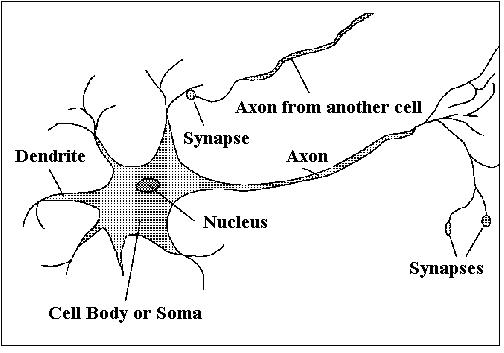
\includegraphics[width=300pt,height=200pt,scale=2]{Pics/neuron.jpg}
\centering
\caption{A neuron}
\end{figure}

One of the most important parts of the neuron structure is the synapse. The synapse is the contact between the axon of a neuron and the dendrite or the soma of another. It is where a information from one neuron is transmitted to the other. When a set of neurons are connected with each other through synapses, then they create a neural network.

Finally, the communication between neurons is accomplihed through spikes, which are either chemichal or electrical\cite{gerstner2002spiking}.

Given the terms in this section, the name of the SpiNNaker chip is detuctable. It stands for Spi(king)N(eural)N(etwork) architecture.
\subsection{The SpiNNaker architecture}
As mentioned before the SpiNNaker architecture is inspired by the biology of the brain, and more specifically, neurons. However, its architecture is not constrained by the biology of the brain, but many techniques to speed up computations are used. It differs from other supercomputers, which  usually have a lot of strong processors with slow network capabilities. The design of the architecture was made with having as priority two concerns. The first one being MIPS(millions of instructions per-second) per mm$^2$. Namely how many instructions can be performed in an area of silicon. The second one was MIPS per watt, which means how many instructions per second can be performed given a fixed amount of energy. Its most optimal configuration will use a million cores and will be able to simulate over a billion neurons\cite{furber2007neural}.
\subsubsection {SpiNNaker chip Overview}
The heart of the SpiNNaker architecture is the SpiNNaker chip. Its main components are 18 identical ARM cores, a router, a system NoC(Network-on-Chip) which connects to the router of the chip and a 128 MB SDRAM. At startup, in each chip a processor is selected to act as a Monitor processor, with the functionality of performing the management of the given chip's system. The remaining ARM cores perform the calculations for the given problem, with the exception of one which is reserved as a spare, in the emergency of another core having a malfunction\cite{furber2007neural}. Each core has the ability to hold 32KB of instructions and 64KB of data. Since this is not enough space, all other data is saved in the SDRAM which can hold up to 1GB of data\cite{navaridas2009understanding}.
\begin{figure}[h!]
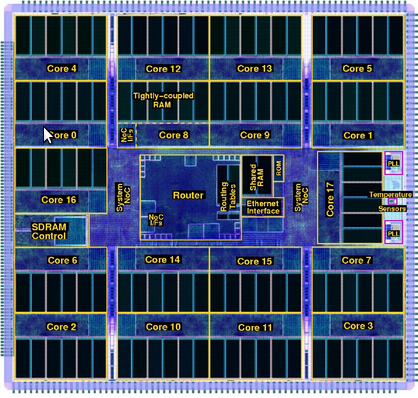
\includegraphics[width=250pt,height=150pt,scale=2]{Pics/chip.png}
\centering
\caption{The SpiNNaker chip\cite{spinnweb}}
\end{figure}
\subsubsection{The router}
As mentioned before the architecture supports low-delay communication, with less powerful processors, than those used in most supercomputers. To accomplish that, the system uses asynchronous multicast packets to communicate between cores. This is done through the router which exists in each chip.

The router exists as the part of the NoC and its primary role is to direct packets that arrive and packets that are sent or need to be forwarded. The router has 20 ports for the ARM cores that are located in the given chip and is able to forward one packet at a time. The router works faster than a transmission port, which results into the router being most of the time lightly used. It is designed to support point-to-point communication, using small packets. Using multicast packets helps reduce the amount of packets that exist in any givne moment in the network. To help with that, the architecture supports default routing, which means that some connections do not need to be in some routing tables for them to be forwarded to their eventual destination. This concept will be explained in the next section.

The functionality of the router is pretty simple. When a packet arrives from the input port, then the router will try to send it to an output port. If there is a problem during transmission, then the router will keep trying to send it and after a while it will try the emergency route(also explained in the next section). If the emergency route still does not work and an amount of time is passed, then the packet will be dropped. To help with that, each packet has the time it was transmitted in their header.

\begin{figure}[h!]
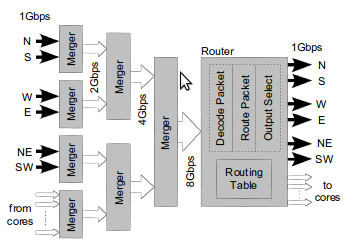
\includegraphics[width=250pt,height=150pt,scale=2]{Pics/router.png}
\centering
\caption{The router\cite{navaridas2009understanding}}
\end{figure}
To further understand this concept, the topology of the system needs to be considered.
\subsubsection{Topology}
In order to have a million cores available for processing a number of SpiNNaker chips need to get connected and work efficiently as an architecture. To reach that goal an effective topology is important.
\begin{figure}[h!]
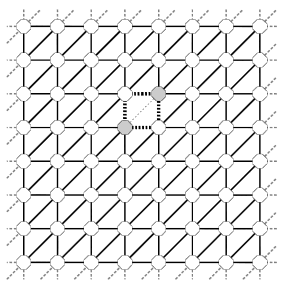
\includegraphics[width=250pt,height=250pt,scale=2]{Pics/topology.png}
\centering
\caption{
\emph{The SpiNNaker topology\cite{navaridas2009understanding}. This is an example of what an 8x8 would look like.Each circle is a SpiNNake chip and the lines between them are the connectivity.}}
\end{figure}
\vspace{20pt}
Considering Figure 4, it is visible that the topology is viewed by the system as a 2D mesh, with chips having a specific amount of neighbours and specific connections. Any chip is able to communicate directly to 6 other chips. This is also depicted in Figure 3, where the positions of these chips are shown. In general each chip directly communicates with chips that are North, South, West, East ,NorthEast, and Southwest of its respective position. This however does not apply for chips that are in the perimeter of the mesh, since they in some of the positions described above chips will not exist. 

Returning now to the default routhing mentioned in the previous section, if a packet arrives to a router, and the router does not have an entry for it, a then it will be forwarded to the chip opposite to the one it came from. For example, if a packet comes from the East and the aforementioned condition is met, then it will be forwarded to the West. This helps reduce the size of the routing tables in each chip\cite{khan2008spinnaker}.

In addition to the default routing, the topology also provides for two-hop routes aming neighbor chips, as shown in Figure 4. These routes are named emergency routes and their functionality is to bypass any faulty connections that might exist between connections.
\newpage
\subsection{The Conjugate Gradient Method}
The conjugate gradient method is an algorithm for the numerical solution of systems of linear eqations of the type Ax=b, those whose matrix is symmetric and positive definite. 

A \emph{symmetric} matrix is a matrix which is equal to its transpose. If A is a symmetric matrix then A=A$^T$. The entries of the matrix are symmetric with respect to the main diagonal, so if an element of the matrix A is a, then a$_{ij}$=a$_{ji}$. 
A \emph{positive definite} matrix M is a matrix which when multipled by any non-zero vector z and its transpose z$^T$, is always positive. In short the relationship that needs to be satisfied is zMz$^T$>0

It is an iterative method, which means it can be applied to sparse systems. A \emph{sparse matrix} is a matrix which is populated primirily with zeros. Its opposite would be a \emph{dense matrix}. It was developed by Magnus Hestenes and Eduard Stiefel and can be used to solve optimization problems\cite{press2007numerical}.
\subsubsection{The quadratic form}
In order to explain why the Conjugate Gradient Method can solve problems whose matrix is positive-definite and symmetric an explanation of the quadratic form needs to be presented.
\begin{center}
\begin{equation}
f(x)=\frac{1}{2}x^TAx-b^T+c
\end{equation}
\end{center}

The gradient $\nabla f(x)$ of the quadratic form is a vector field that points in the direction of the greatest increase of $f(x)$. If we were to take into account the i$^{th}$ component of $\nabla f$, then.
\begin{equation}
\begin{split}
f(x+\psi e_i)= \frac{1}{2} (x+\psi e_i)^TA(x+\psi e_i)-b^T(x+\psi e_i)+c\\
= \frac{1}{2} (x^TAx+\psi e^T_iAx +x^TA\psi e_i)-b^T(x+\psi e_i)+c
\end{split}
\end{equation}
Note that e$_i$ is the error affiliated with taking the i$^{th}$ component of $\nabla f$. Now from the definition of a derivative $f(x)$=$\frac{f(a+h)-f(a)}{h}$ and (2) we have.
\begin{equation}
\frac{f(x+\psi e_i)-f(x)}{\psi}=\frac{\frac{1}{2}(\psi e^T_iAx+x^TA\psi e_i)-\psi e^T_ib}{\psi}
\end{equation}
(3) is the same as the i$^{th}$ component of $\frac{1}{2}$(Ax+A$^T$x)-b
So we have
\begin{equation}
\nabla f =\frac{1}{2}A^Tx+\frac{1}{2}Ax-b
\end{equation}
But if A is symmetric, then it is obvious that we have $Ax=b$ at the minimum of $f$. In addition if A is positive negative then $f$ is concave up.
\subsubsection{Conjugate Gradients}
As mentioned before the matrix A must be symmetric and positive definite for the Conjugate Gradient Method to work. Given a quadratic function 
as defined in (1), then it turns out that $-\nabla f=b-Ax=r$.

The CGM, as well as most optimization methods(for example the method of the Steepest Descent\cite{rosenbloom1956method}), look towards a specific direction everytime they are to move to a correct position and try to look for the best step given their gradient and direction
\begin{equation}
x_{k+1} = x_k + \alpha p_k
\end{equation}
Given (5), $\alpha$ can be deduced from the fact that $e_{k+1}$(the error vector of each iteration) must be orthogonal to p$_k$,  which also means that p$_k$ will never be met again as the solution progresses. Using this we can dedcuce
\begin{equation}
\begin{split}
p^T_ke_{k+1}=0\\
p^T_k(e_k+\alpha p_k)=0\\
\alpha = -\frac{p^T_ke_k}{p^T_kp_k}
\end{split}
\end{equation}

The equation at (6) however is not solvable. The value of $e_k$ is needed in each iteration, which is not computable at that time. To help with that the search directions in each iteration($p_k$) is defined as A-orthogonal in respect to the matrix A, instead of just orthogonal. The definition of A-orthogonal vectors is, given a matrix A, then:
\begin{equation}
p^T_kAp_k=0
\end{equation}
Given (7), $e_{k+1}$ and $p_k$ must be A-orthogonal. If we wish to find the optimal value for $\alpha$,then the gradient must be set to 0. This leads to the following equation.
\begin{equation}
0=\frac{d}{d\alpha}f(x_{k+1})=\nabla f(x_{k+1})^T\frac{d}{d\alpha}x_{k+1} = -r^T_{k+1}\frac{d}{d\alpha}(x_k + \alpha p_k) = -r^T_{k+1}p_k=p^T_kAe_{k+1}
\end{equation}
From (6),(7) the equation for $\alpha$ when $e_k$ and $p_k$ are A-orthogonal is
\begin{equation}
\begin{split}
\alpha =-\frac{p^T_kAe_k}{p^T_kAp_k}\\
=\frac{p^T_kr_k}{p^T_kAp_k}
\end{split}
\end{equation}

Another important equation that comes from analysing the error term is
\begin{equation}
p^T_kr_k=u^T_kr_k
\end{equation}

In (10) $u^T_k$ are u vectors that span the vector subspace of the vector field of $p_k$. They are also orthogonal to $r_k$ and $u_{k+1}$ is also orthogonal to all the previous $u$ vectors.

Using (9) and (10) we are able to reach a more accurate value for $\alpha$
\begin{equation}
\alpha = \frac{r^T_kr_k}{p^T_kAp_k}
\end{equation}

Using (9) and (10) and a Gram-Schmidt conjugation we are able to reach and a value for $\beta$
\begin{equation}
\beta = \frac{r^T_{k+1}r_{k+1}}{r^T_kr_k}
\end{equation}
\newpage
\subsubsection{The algorithm}
Combining the optimal value of $\alpha$(8) and $\beta$(9) and a good step direction for p$_k$ the Conjugate Gradient Method is formed as follows
\\
\begin{algorithmic}
\STATE r$_0$=b-Ax$_0$
\STATE p$_0$=r$_0$
\STATE k=0
\FOR{k to 1000000}
\STATE $\alpha_k=\frac{r_k ^T*r_k}{p_k ^T*A*p_k}$
\STATE x$_{k+1}$=x$_k$+$\alpha_k$*p$_k$
\STATE r$_{k+1}$=r$_k$-$\alpha_k$*p$_k$*A
\IF{r$_{k+1}^T$*r$_{k+1}$ is small enough}
\STATE break
\ENDIF
\STATE $\beta_k=\frac{r_{k+1} ^T*r_{k+1}}{r_k ^T*r_k}$
\STATE p$_{k+1}$=r$_{k+1}$+$\beta_k$*p$_k$
\STATE k=k+1
\ENDFOR
\end{algorithmic}
\vspace{20pt}
Some notes that can be made about this algorithm are that the axis is defined by the eigenvectors of A and that the algorithm takes a conjugate step closest to $r$. Finally, the algorithm guarantees convergeance in at most n steps.\cite{press2007numerical}\cite{shewchuk1994introduction}\cite{cgm2009lec}

Ofcourse there is an error that exists in every step, as mentioned before, but it is minimized in each iteration. The error function would be:
\begin{equation}
\begin{vmatrix}
e_k
\end{vmatrix}
\leq 2(\frac{\sqrt{\kappa}-1}{\sqrt{\kappa}+1})^k
\begin{vmatrix}
e_0
\end{vmatrix}_A
\end{equation}

In Equation 9 $\kappa$ is the condition number.

Another interesting applicatoin of the Conjugate Gradient Method is that you can apply precondition on it in order to find the solution faster. However, preconditioning is outside of the scope of this project, since it adds a lot more calculation and would need a less general solution.
\subsubsection{Parallel solutions of the CGM}

Some parallel implementations of the CGM use blocks of the input vectors and matrix and assign them carefully to specific cores, thus letting each core produce output that will be used in the next iteration. These kinds of solutions work better with vector processors, since it allows a processor to complete large vector operations. Depending on how many processors a machine has, parts of the algorithm can continue being sliced to blocks, until the optimal implementation is reached\cite{o1987parallel}.

Some other parallel implementations try to use more specific preconditionings to achieve faster results, but again for the parallel part, they split the input into blocks to distribute it to various cores\cite{adams1985m}\cite{adams1983m}. 

One of the most interesting implementations of the CGM, suggests an improved algorithm named ICGS(Improved Conjugate Gradient Squared), which is based in another already altered version of the CGM\cite{maheswaran1999mcgs}. This implementation computes all vector-matrix  multiplications and inner products concurrently, for each iteration. The communication time between these operations and vector updates has been organised efficiently, so that global communication drops significantly, thus dropping the run time of the algorithm as well\cite{yang2001improved}.

Finally, there are many recent implementations which have used GPU's in order to solve the Conjugate Gradient Method efficiently. These pieces of work use CUDA and various other techniques to accomplish their goal, with some very good results. Ofcourse different GPU models are used, but that just enhances the generality of the solution. Generally though,as is for most parallel implementations of the CGM, the most used technique is reducing the time it takes to compute the matrix-vector multiplication and inner products, thus reducing the time of the algorithm overall\cite{galiano2012gpu}\cite{wozniak2010parallel}.
\newpage
\bibliographystyle{plain}
\bibliography{ref.bib}
\cite{navaridas2009understanding}
\cite{sharp2012power}
\cite{davies2010interfacing}
\cite{sharp2011event}
\cite{gerstner2002spiking}
\cite{press2007numerical}
\cite{shewchuk1994introduction}
\cite{cgm2009lec}
\cite{o1987parallel}
\cite{adams1985m}
\cite{maheswaran1999mcgs}
\cite{yang2001improved}
\cite{adams1983m}
\cite{galiano2012gpu}
\cite{wozniak2010parallel}
\cite{hestenes1952methods}
\cite{rosenbloom1956method}
\cite{furber2007neural}
\cite{spinnweb}
\cite{khan2008spinnaker}
\end{document}